\documentclass[acmtog, authorversion]{acmart}

\usepackage{booktabs} % For formal tables

% TOG prefers author-name bib system with square brackets
\citestyle{acmauthoryear}
\setcitestyle{square}


\usepackage[ruled]{algorithm2e} % For algorithms
\renewcommand{\algorithmcfname}{ALGORITHM}
\SetAlFnt{\small}
\SetAlCapFnt{\small}
\SetAlCapNameFnt{\small}
\SetAlCapHSkip{0pt}
\IncMargin{-\parindent}

% Metadata Information
%\acmJournal{TOG}
%\acmVolume{9}
%\acmNumber{4}
%\acmArticle{39}
%\acmYear{2010}
%\acmMonth{3}

% Copyright
%\setcopyright{acmcopyright}
%\setcopyright{acmlicensed}
%\setcopyright{rightsretained}
%\setcopyright{usgov}
\setcopyright{usgovmixed}
%\setcopyright{cagov}
%\setcopyright{cagovmixed}

% DOI
%\acmDOI{0000001.0000001_2}

% Paper history
%\received{February 2007}
%\received{March 2009}
%\received[final version]{June 2009}
%\received[accepted]{July 2009}


% Document starts
\begin{document}
% Title portion
\title{SketchingPhoto: Progressively draw a realistic photo} 

\author{Author}



\begin{abstract}
Abstract <TODO>
\end{abstract}


%
% The code below should be generated by the tool at
% http://dl.acm.org/ccs.cfm
% Please copy and paste the code instead of the example below. 
%
%\begin{CCSXML}
%<ccs2012>
% <concept>
%  <concept_id>10010520.10010553.10010562</concept_id>
%  <concept_desc>Computer systems organization~Embedded systems</concept_desc>
%  <concept_significance>500</concept_significance>
% </concept>
% <concept>
%  <concept_id>10010520.10010575.10010755</concept_id>
%  <concept_desc>Computer systems organization~Redundancy</concept_desc>
%  <concept_significance>300</concept_significance>
% </concept>
% <concept>
%  <concept_id>10010520.10010553.10010554</concept_id>
%  <concept_desc>Computer systems organization~Robotics</concept_desc>
%  <concept_significance>100</concept_significance>
% </concept>
% <concept>
%  <concept_id>10003033.10003083.10003095</concept_id>
%  <concept_desc>Networks~Network reliability</concept_desc>
%  <concept_significance>100</concept_significance>
% </concept>
%</ccs2012>  
%\end{CCSXML}

%\ccsdesc[500]{Computer systems organization~Embedded systems}
%\ccsdesc[300]{Computer systems organization~Redundancy}
%\ccsdesc{Computer systems organization~Robotics}
%\ccsdesc[100]{Networks~Network reliability}

%
% End generated code
%


\keywords{GANS, sketch}


\maketitle

\section{Introduction}
\subsection{Motivation and Goal}
In many applications such as movie making, public security, and so on, virtual images are desired from sketches or several words describing the target object. Typically, an \textbf{interactive process} is employed to generate images, collect feedbacks, and then providing more information to keep updating the output image.

Possible directions:
\begin{enumerate}
	\item \textbf{SketchingAPhoto} Based on the image-image translation work, we can link hand-drawn sketch to edge map first, and then generate photo from the edge map. Step 1: retrieve similar edge maps by the input sketch; Step 2: generate images from the retrieved edge map.
	%
	\item \textbf{Face Image generation by text} while somebody is asked to describe a suspect, how to generate a photo/literary sketch to based on texts. How do people describe human faces. How do experts produce a sketch based on the words? 
\end{enumerate}


\subsection{Image-to-image translation}
Image-to-image translation has drawn a lot of attention recently, which aims to apply an image in one domain to generate a corresponding image in another, reserving shared concepts, objects or scenes in these two images.  

Generating a corresponding image from an input image can be reformulated as a conditional image generation problem which is conditioned on the input image. Previous works about conditional image generation problem focused on generating images from discrete labels~\cite{CGAN}, texts~\cite{Reed2016} and images.
\cite{pix2pix} firstly introduced the concept of image-to-image translation and trained a framework by paired images to handle multiply applications, such as labels to street scene, day to night, edge to photo and etc., only switching the training datasets.
%
\cite{CycleGAN, DiscoGAN, UNIT} extend the translation with difficultly and expensively achieved paired image datasets to unpaired image datasets, and they hugely widened the application to cover the scene where the desired outputs are highly complex or not even well-defined.

However, the previous works share a common shortage that the generated images always reserve the edge layout of the input images. 

\section{Related work}
\subsection{Sketch}
Sketches has been well studied in past years. \cite{HowToSketch} released a large sketch dataset with 20K sketches in 250 categories and proposed a sketch classigfication method based on a bag-of-feature sketch representation and multi-class support vector machines. 
%
\cite{SketchANet} achieved a sketch classification performance surpassing that of humans by developing two data augmentation strategies to significantly increase the volume and diversity of sketches and exploring different network ensemble fusion strategies to improve the classification performances.
\cite{Sketch3DShape} introduced a sketch-based 3D shape retrieval method that trained two siamese convolutional neural networks to learning the views for 3D shape and the sketches.
Unlike works prior to it which have retrieved images in the same category of the query sketch, \cite{SketchMeThatShoe} addressed a fine-grained sketch-based image retrieval problem that required instance-level retrieval of images. They trained a siamese networks with a newly collected dataset of sketch-photo pairs and applied staged pre-training and fine-tuning.

\subsection{Conditional Generative Adversarial Networks}
Our work is based on generative adversarial networks (GANs)~\cite{GAN} in conditional setting. 

Previous works have explored GANs generating images in the condition of discrete labels~\cite{CGAN}, text~\cite{Reed2016} and images. 
Conditional GANs were firstly introduced by \cite{CGAN} who treated the conditional generation problem as the inverse processing of image classification and used discrete labels as condition to generate images.
%
\cite{Dosovitskiy2014} trained convolutional networks to generate images of objects given object style, viewpoint and color. With the experiments of interpolating viewpoints, they showed that networks learn a meaningful representation of 3D models. 
%
\cite{Reed2016} generated photo-realistic images conditioned on text descriptions.

\subsection{Image-to-image translation with GANs}
Given an image in one domain, image-to-image translation methods generate a corresponding image in another. These two images are possible representations of the same scene. Image-to-image translation with GANs is a special case of conditional GANs where images are applied to be conditions. 
%

\cite{pix2pix} firstly introduced the concept of image-to-image translation, who treated one image in a paired image dataset as conditioned input and generate its corresponding image. Unlike works prior to it which dealt with only one application, \cite{pix2pix} are able to handle multiple applications in one frame work only switching training datasets. They applied skip connections between mirrored layers in the generator to make sure low-level information pass through its encoder-decoder architecture and used dropout in stead of random vector to provide stochasticity in the networks.
%
\cite{UNIT} studied on unpaired image-to-image translation by training a two-branch GAN. Each branch is composed with a encoder, a generator and a discriminator. With the idea that high-level representation of a pair of corresponding images in two domains should be the same, high-level layers share weights between two branches in encoders, generators and discriminators. 
%

CycleGAN~\cite{CycleGAN}, DiscoGAN~\cite{DiscoGAN} and DualGAN~\cite{DualGAN} developed similar architectures to translate unpaired images which contain, for each, two generators and two discriminators. These methods learn two mappings in an adversarial training process such that an input image in one domain is mapped to a generated image in another, and then the generated image is mapped to a reconstructed image which is closed to the input image in some measures. These methods shared the same idea that since the generated image is able to reconstruct the input image, it should contain the content of the input image.
\section{SketchingAPhoto Exploration}
Based on the image-image translation work, we can link hand-drawn sketch to edge map first, and then generate photo from the edge map. Step 1: retrieve similar edge maps by the input sketch; Step 2: generate images from the retrieved edge map.
\subsection{Linking sketches to edge maps}
The idea of linking a sketch to an edge map can be treated as either a sketch-based edge maps retrieval problem or a sketch-based edge maps generation problem .
\paragraph{Sketch-based edge maps retrieval}
If we have edge maps to be retrieved, we must have their corresponding images.Since sketch-based image/photo retrieval is well studied, we can separate sketch-based edge maps retrieval into two part: sketch-based image retrieval and edge detection. \cite{SketchMeThatShoe} is an instance-level sketch-based image retrieval method using a novel data augmentation technique and a pre-trained triplet convolutional neural network (Figure~\ref{reported_sketchmethatshoe}). On a newly collected chairs-sketches dataset, top-1 accuracy is $69.07\%$ and top-10 accuracy is $97.94\%$. On another dataset of shoes and sketches, top-1 accuracy is $39.13\%$ and top-10 accuracy is $87.83\%$. An edge detection algorithm will be introduced in next subsection. To test this idea, we are training an edge2shoe translation model.
\paragraph{Sketch-based edge maps generation}
Sketch-based edge maps generation is a special case of image-to-image translation or style transfer, while in this case, both sketches and edge maps are lack of textures and colors, which might make this task more challenging. 
To be explored...

\begin{figure}
	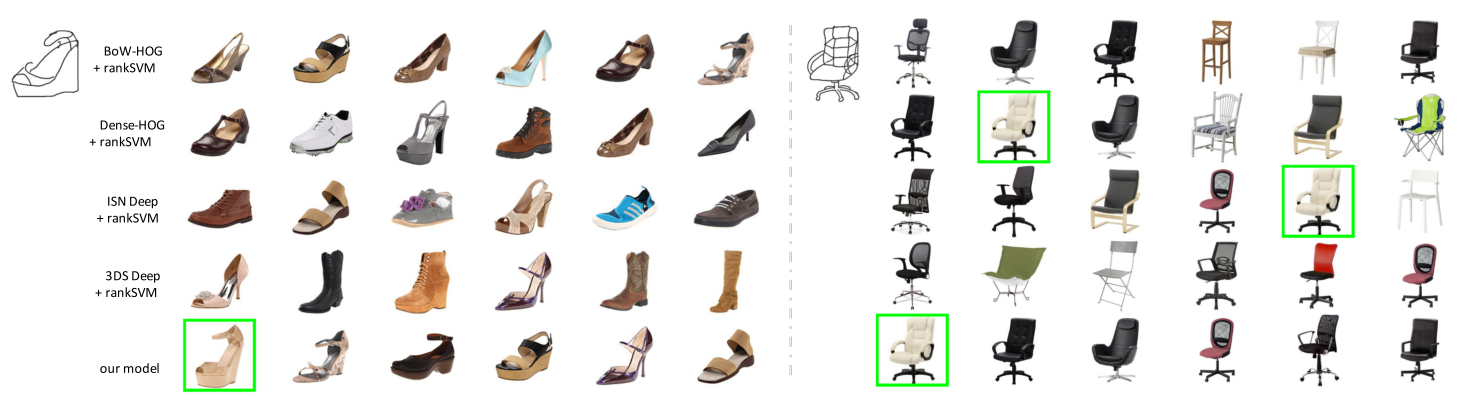
\includegraphics[width=\textwidth]{figures/pix2pix/reported_sketchmethatshoe}
	\caption{\label{reported_sketchmethatshoe}Reported Ranking examples using different compared models. The true matches are highlighted in green. Results on last row are of \cite{SketchMeThatShoe}}
\end{figure}

\subsection{Edge map to photo translation}
Pix2pix~\cite{pix2pix} introduced an algorithm to train a GAN-based model with image pairs to translate an image in one domain to a corresponding in another. Edge-to-photo translation is one of its applications, which needs to train the model with photos of the same category and their edge maps. We examined this method on tasks of edge2cat, in which we use a set of cat photos and corresponding edge maps to train the model. Hyper-parameters are all the same as the reported in the pix2pix paper.
\subsubsection{Details}
\paragraph{Dataset}
We downloaded 1831 photo images of the cat category from ImageNet~\cite{ImageNet} as our photo images. These images are cropped to the size of $256\times 256$. And then we extracted the edge maps of these images using holistically-nested edge detection (HED) as suggested by pix2pix. 
\paragraph{Edge Detection}
HED is a new edge detection algorithm, which performs image-to-image prediction by means of a deep learning model that leverages fully convolutional neural networks and deeply-supervised nets. HED automatically learns rich hierarchical representations (guided by deep supervision on side responses) that are important in order to resolve the challenging ambiguity in edge and object boundary detection. Postprocessing is conducted to remove short edges and convert HED edge maps to be binary.
\paragraph{Performance}
We compared results of edge2cat (Figure~\ref{pix2pix_edge2cat}) with the reported results. The results on edge2cat, which can easily be distinguished from realistic photos, are not as good as those on edge2handbag (Figure~\ref{pix2pix_edge2handbag}) and edge2shoe (Figure~\ref{pix2pix_edge2shoe}). It seems to be because that the criteria of realistic on cats are more rigid than those on handbags and shoes, especially around the eyes of cats. Also the backgrounds of cat images bring more challenges while in the shoes and handbag images the backgrounds are all white, which make the edge maps of cats much more complicated and edge2cat model harder to train. Moreover, compared to the results of edge2cat posed on the git repository (Figure~\ref{pix2pix_reported_edge2cat}), the model we trained fails to generate eyes of cats. 
\subsection{Discussion}
We now have at least three paths to achieve our goal of sketching a photo. 
\paragraph{Sketch-based edge maps retrieval plus edge2photo translation}
Given some well-studied fruits such as sketch-based image retrieval and edge2photo translation, this method might be the easiest one compared to the other two. However, it is uncomfortable to me .
To be simple, this method can be described as "sketch--retrieved image--edge map--generated photo". 
The motivation seems not clear. It seems the generated photo should be the same as the retrieved image. If someone wants to get the generated photo, the retrieved image might be what he wants. 
\paragraph{Sketch-based edge maps generation plus edge2photo translation}
We have not explored this path. As discussed above, both sketches and edge maps are lack of textures and colors. Due to high intra-class variation and iconic style, the semantic information might be harder to extract. The HED algorithm might give us some hints. More survey is needed.
\paragraph{Sketch2photo translation}
An photo generation method conditioned on sketched with/without the help of edge maps. It should more challenging. This will be explored in next subsection.



\begin{figure}
	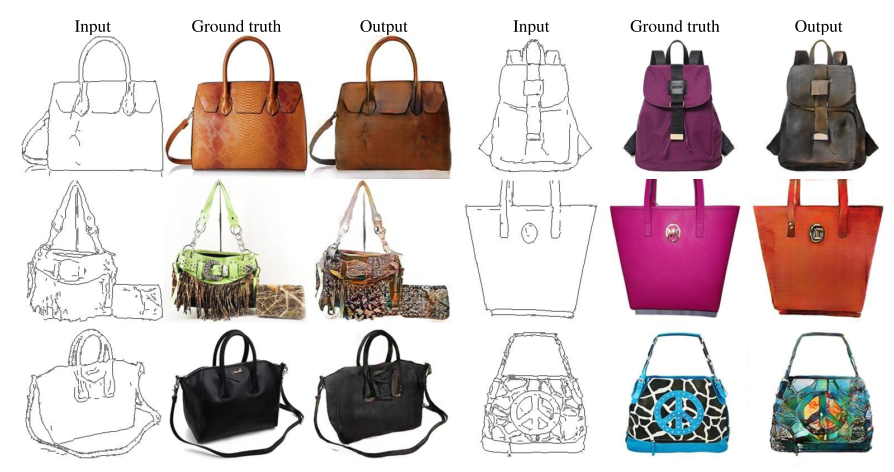
\includegraphics[width=0.5\textwidth]{figures/pix2pix/reported_edge2handbag}
	\caption{\label{pix2pix_edge2handbag}Reported results on edge2handbag of pix2pix.}
\end{figure}
\begin{figure}
	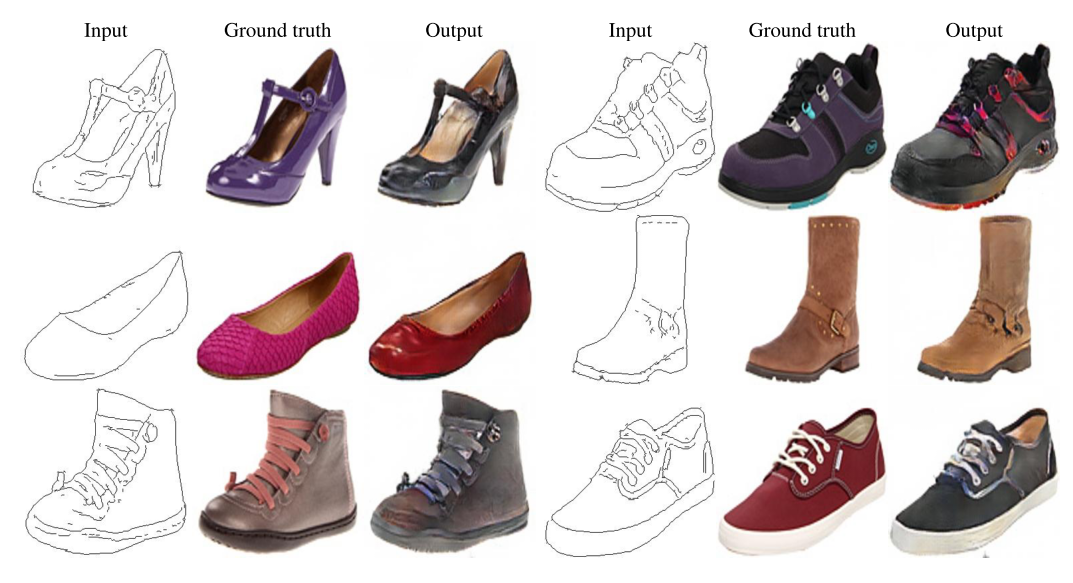
\includegraphics[width=0.5\textwidth]{figures/pix2pix/reported_edge2shoe}
	\caption{\label{pix2pix_edge2shoe}Reported results on edge2shoe of pix2pix.}
\end{figure}

\begin{figure}
	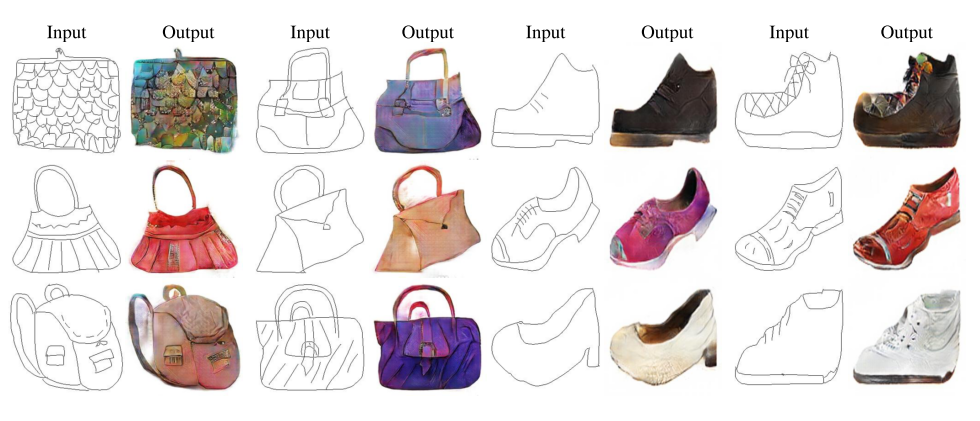
\includegraphics[width=0.5\textwidth]{figures/pix2pix/reported_sketch2handbag}
	\caption{\label{pix2pix_sketch2shoeNhandbag}Reported results on sketch2handbag and sketch2shoe of pix2pix.}
\end{figure}

\begin{figure}
	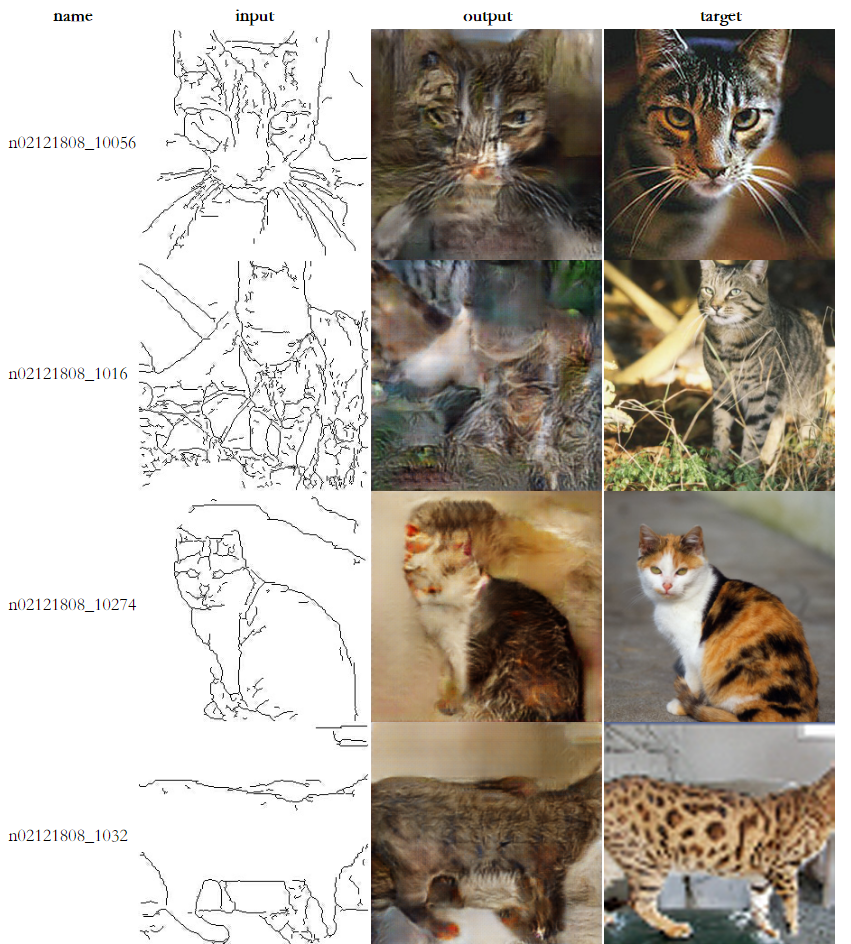
\includegraphics[width=0.5\textwidth]{figures/pix2pix/edge2cat}
	\caption{\label{pix2pix_edge2cat}Pix2pix results on edge2cat trained by our collected cat images and their edge maps. The model we trained fails to generate photos as realistic as edge2shoe and edge2handbag tasks. $\gamma = 25.0/255.0$}
\end{figure}
\begin{figure}
	\includegraphics[width=0.5\textwidth]{figures/pix2pix/edge2photo/gamma_5/results.png}
	\caption{\label{pix2pix_edge2cat_gamma5}Pix2pix results on edge2cat trained by our collected cat images and their edge maps. $\gamma = 5.0/255.0$}
\end{figure}
\begin{figure}
	\includegraphics[width=0.5\textwidth]{figures/pix2pix/edge2photo/grayscale/200/results.png}
	\caption{\label{pix2pix_edge2cat_gray_200}Pix2pix results on edge2cat trained by our collected cat images and gray-scale edge maps.}
\end{figure}

\begin{figure}
	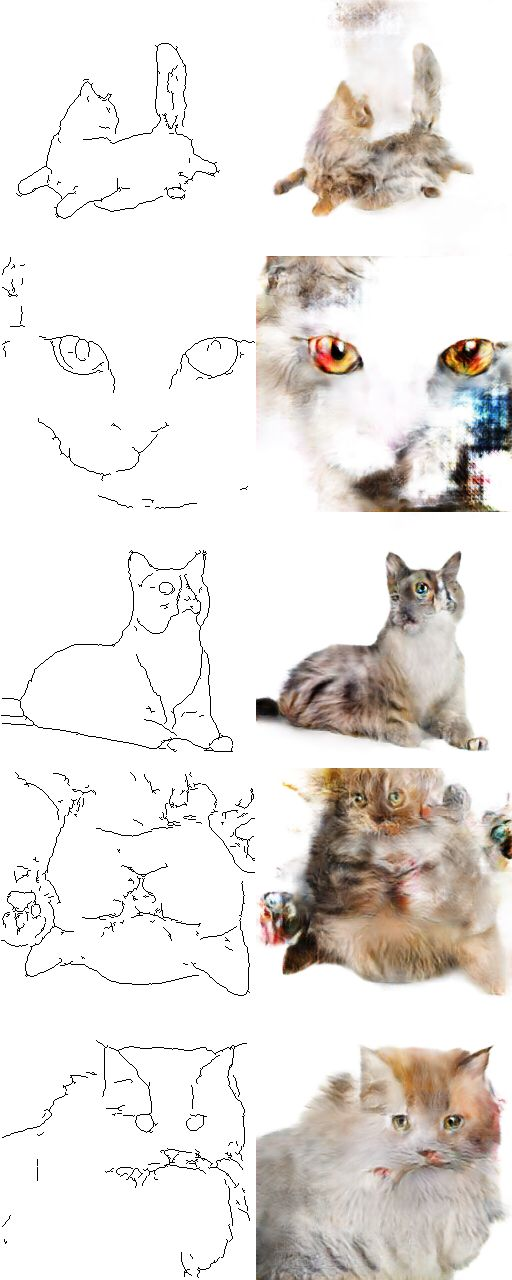
\includegraphics[width=0.4\textwidth]{figures/pix2pix/edges2cats-sheet}
	\caption{\label{pix2pix_reported_edge2cat}Pix2pix results on edge2cat posed on the git repository.}
\end{figure}

\subsection{CycleGAN}
CycleGAN is image-to-image translation algorithm trained by unpaired images of two domains.
\subsubsection{Details}
\paragraph{Residual blocks}
In spired by \cite{Johnson et. al.}, in the bottleneck layers, residual blocks~\cite{ResNets} are added to transfer features of input image to features of generated image. 
\paragraph{Instance normalization}
Instance normalization is also unknown as contrast normalization. CycleGANs swap batch normalization with instance normalization in both training and testing time since we want to keep the content instead of style and contract is clearly not a part of content in the image.
\paragraph{Generated image pool}
CycleGANs discard both random vectors and dropout which introduce stochasticity in the training procedure and use the historical generated images to update the discriminators by maintaining a generated image pool with size of 50. The pool is filled with first generated 50 images and updated by replacing one of randomly selected images in it with the newly generated image.
%
\begin{figure}
	
	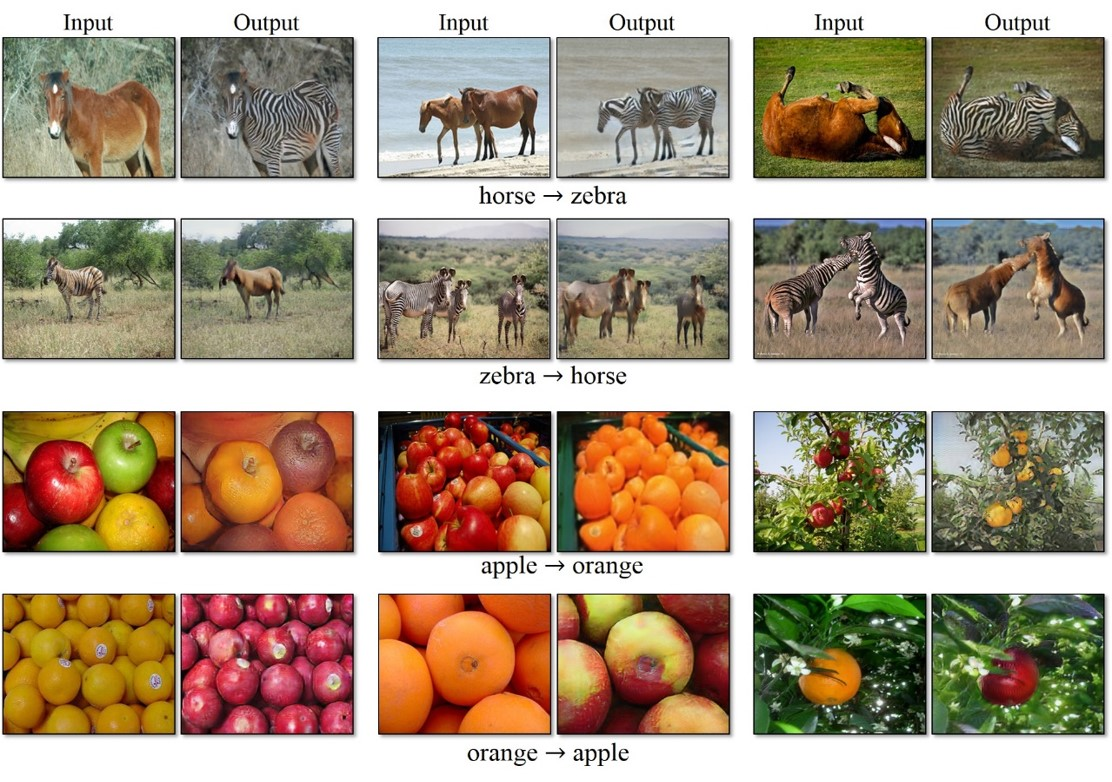
\includegraphics[width=0.5\textwidth]{figures/cyclegan/reported_results.jpg}
	\caption{\label{cyclegan_reported_results}Reported results of CycleGAN.}
\end{figure}
%
\begin{figure}
	
	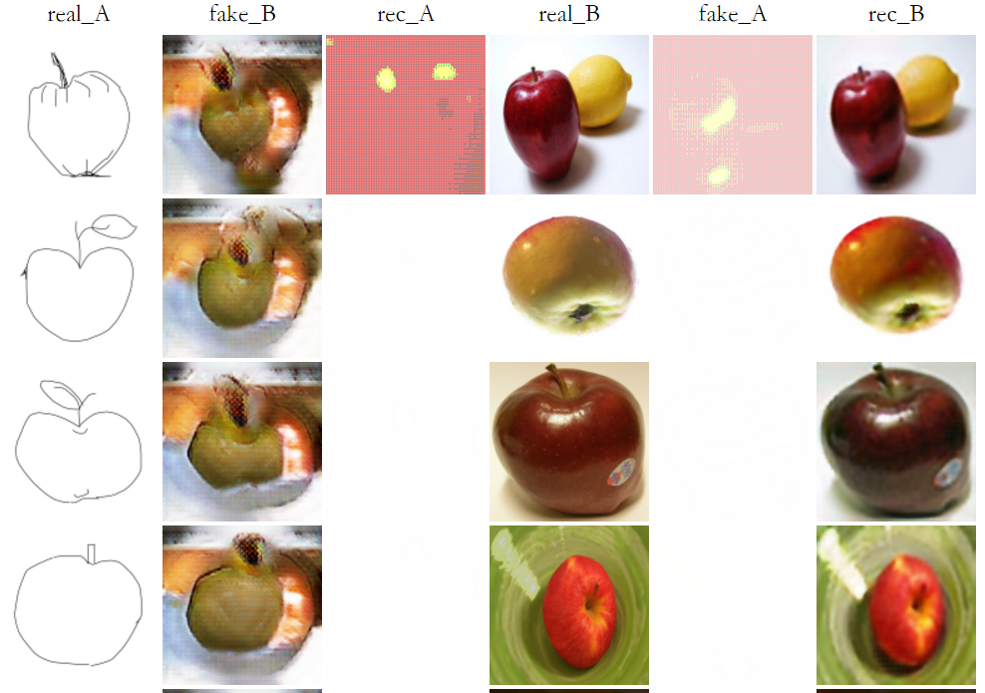
\includegraphics[width=0.5\textwidth]{figures/cyclegan/sketch2photo_apple_200epochs_torch.png}
	\caption{\label{cyclegan_sketch2photo_apple}Results of CycleGAN on sketch-to-photo dataset of apples. Mode collapse problem is severe and reconstructed images are "almost white".}
\end{figure}
%
\begin{figure}
	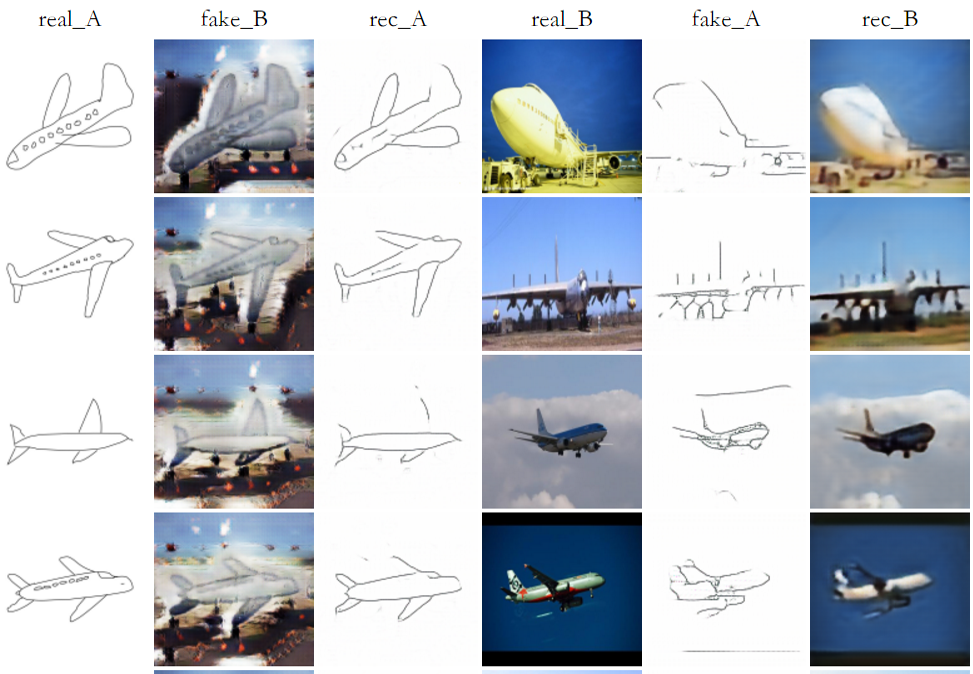
\includegraphics[width=0.5\textwidth]{figures/cyclegan/sketch2photo_airplane_200epochs_torch.png}
	\caption{\label{cyclegan_sketch2photo_airplane}Results of CycleGAN on sketch-to-photo dataset of airplanes. Mode collapse problem is severe.}
\end{figure}
%
%
\subsubsection{Results of sketch-to-photo translation}
Figure~\ref{cyclegan_reported_results} shows the reported results of CycleGAN. Notice that, taking horse-to-zebra as example, only the horse in the input image rather than the whole image is translated into black and white, which is different from style transfer where the styles of both the object and background are transfered. Also, the green grass in the background is translated into brown, the color of the environments zebras live in.

However, when we train CycleGAN with the sketch-to-photo dataset ("real\_A" and "real\_B" in figure~\ref{cyclegan_sketch2photo_apple} and ~\ref{cyclegan_sketch2photo_airplane}, results are not as good as the other. As illustrated, both models suffer from severe issue of mode collapse, a common but unsolved problem of training GANs that input images of different modes are mapped to images of the same mode in corresponding domain. Also, the edges of the input images are preserved in the generated images. This is acceptable in some application like horse-to-zebra or apple-to-orange, since the contours of the the input objects and output objects are similar to each other. However, when it comes to the sketch-to-photo, the preserving of edges is unexpected since objects in generated photos with free-hand style contours are not visually real.

\subsection{Assessment of image quality}
A straightforward metric of performance of the generated images can be the judge of human. However, this is labor-intensive. Another metric named Inception score is proposed in \cite{ImprovedTechnique} which applies Inception model to every generated image to get the conditional and marginal label distribution and uses the KL divergence between these two distributions as the metric: $exp\{\mathcal{E}_x{KL(p(y|x)||p(y))}\}$. The insight of this metric is that the conditional label distribution should have low entropy (one-hot like) because something must be detected in the input image to make it realistic, while the marginal distribution should have high entropy (uniform like) because they want various kinds of images.

Since our training dataset contains images with only one class of label, we do not want the marginal distribution have high entropy. We use the entropy of the conditional label distribution 
as the performance metric: $exp\{-\mathcal{E}_x{p(y|x)\log(p(y|x))}\}$.

\subsection{Gray-scale edge map to photo translation using pix2pix}
Given a three-channel image, HED edge detector generates a edge matrix with size as the input image, whose each pixel indicates the probability of being edge in this position of input image. And the post-processing convert the edge matrix into a binary, single-pixel thin edge using a threshold $\gamma$ and non-maximum suppression. Figure~\ref{pix2pix_edge2cat} and figure~\ref{pix2pix_edge2cat_gamma5} shows results of pix2pix trained by binary edge maps with $\gamma=25.0/255.0$ and $\gamma=5.0/255.0$ respectively. We can see that more details are kept in binary edge maps when $\gamma$ is small. 
Also, we train pix2pix with the edge matrices which preserve all details of the edge maps but consist of thick edges. The edge matrices ranging $[0,1]$ are scale to $[0,255]$ to be gray-scale edge maps. Results are shown in figure~\ref{pix2pix_edge2cat_gray_200}. The performances measured by entropy are shown in Table~\ref{pix2pix_performance_metric}.

Generated images with complicated background are much worse. We plan to remove the background of cat images with the help of semantic segmentation method. To be done.
\begin{table}[h]
    \centering
    \begin{tabular}{|l|c|}\hline
    	Images&Entropy\\\hline
    	Training photo images & $0.04463\pm 0.005545$ \\
    	Testing photo images & $0.046676\pm 0.011504$ \\
    	Generated by binary edge maps ($\gamma=25/255$)& $0.013381\pm 0.001917$\\
    	Generated by binary edge maps ($\gamma=5/255$)& $0.017366\pm 0.002494$\\
	    Generated by gray-scale edge maps & $ 0.015774\pm 0.001926$ \\\hline
    \end{tabular}
    \caption{Performances of edge2photo using different training edge maps. The binary edge maps with smaller binary threshold $\gamma$ can generate better images. (More models with different thresholds are training.)}
    \label{tab:pix2pix_performance_metric}
\end{table}


\bibliographystyle{ACM-Reference-Format}
\bibliography{sketch} 

\end{document}
